\documentclass{beamer}
\usepackage{appendixnumberbeamer}

\setbeamertemplate{navigation symbols}{}
\setbeamertemplate{bibliography item}{}
\setbeamerfont{myTOC}{series=\bfseries,size=\Large}
\AtBeginSection[]{\frame{\frametitle{Outline}%
        \usebeamerfont{myTOC}\tableofcontents[current]}}

\renewcommand\footnoterule{} % get rid of line above footnote
\setbeamerfont{footnote}{size=\tiny}

\usepackage{listings}
\usepackage{multicol}
\lstdefinelanguage
   [x64]{Assembler}     % add a "x64" dialect of Assembler
   [x86masm]{Assembler} % based on the "x86masm" dialect
   % with these extra keywords:
   {morekeywords={CDQE,CQO,CMPSQ,CMPXCHG16B,JRCXZ,LODSQ,MOVSXD, %
                  POPFQ,PUSHFQ,SCASQ,STOSQ,IRETQ,RDTSCP,SWAPGS, %
                  rax,rdx,rcx,rbx,rsi,rdi,rsp,rbp, %
                  r8,r8d,r8w,r8b,r9,r9d,r9w,r9b, %
                  r10,r10d,r10w,r10b,r11,r11d,r11w,r11b, %
                  r12,r12d,r12w,r12b,r13,r13d,r13w,r13b, %
                  r14,r14d,r14w,r14b,r15,r15d,r15w,r15b}} % etc.

\usepackage{xcolor}
\definecolor{pale-red}{HTML}{FFCCCC}
\definecolor{pale-yellow}{HTML}{EEEEBB}
\definecolor{pale-green}{HTML}{CCDDAA}

\usepackage{tikz}
\usetikzlibrary{chains}
\usetikzlibrary{shapes.geometric}
\tikzset{box/.style = {draw, rounded corners, on chain, align=center, text centered}}
\tikzset{start/.style = {draw, rounded corners, on chain, align=center, text centered, fill=pale-green}}
\tikzset{stop/.style = {draw, rounded corners, on chain, align=center, text centered, fill=pale-red}}
\tikzset{decision/.style = {draw, rounded corners, on chain, align=center, text centered, fill=pale-yellow}}
\tikzset{arr/.style = {very thick, -latex}}

\usetheme{CambridgeUS} 
\usecolortheme{beaver}

\title[Fuzzing Workshop]{Fuzzing for Automated Vulnerability Discovery}
\author{Lisa Overall}
\date{02 February 2024}

\begin{document}

\frame{\titlepage}

\begin{frame}
\frametitle{Outline}
\tableofcontents
\end{frame}


\section[Motivation]{Motivation}

\begin{frame}
\frametitle{What are the components of a program?}
	
	\begin{itemize}
		\item{Input drawn from some input space (e.g., stdin, network state)}
		\item{States + transitions between them}
		\item{Outputs and/or side effects}
		\item{Termination conditions}
	\end{itemize}

	\centering \includegraphics[scale=.45]{program}

\end{frame}

\begin{frame}
	\frametitle{Software security in a nutshell}
	\LARGE{
	Two important questions:
	\begin{enumerate}
		\item{What inputs cause ``bad" behavior?}
		\item{When is a state ``bad"?}
	\end{enumerate}
	}
\end{frame}

\begin{frame}
	\frametitle{Security engineering (simplified)}

	\begin{columns}[onlytextwidth]
		\begin{column}{.5\textwidth}

			\textbf{Unrestricted input} 
		\begin{itemize}
			\item{Anything can happen}
			\item{Minimal understanding of what code ``should" do}
		\end{itemize}
		\end{column}
		
		\begin{column}{.5\textwidth}
		\centering \includegraphics[scale=.43]{unrestricted}
		\end{column}
	\end{columns}
	
	\pause
	\vspace{.5\baselineskip}

	\begin{columns}[onlytextwidth]
		\begin{column}{.5\textwidth}
			\textbf{Option 1: Restrict inputs} \begin{itemize}
		\item{Typed language}
		\item{Delete code}
		\item{Privilege separation}
	\end{itemize}
		\end{column}
		\begin{column}{.5\textwidth}
			\centering \includegraphics[scale=.5]{restricted}
		\end{column}
	\end{columns}

\pause
	\vspace{.5\baselineskip}

	\begin{columns}[onlytextwidth]
		\begin{column}{.5\textwidth}
	\textbf{Option 2: Test inputs} \begin{itemize}
		\item{Unit tests}
		\item{Fuzzing}
		\item{Property tests}
	\end{itemize}
		\end{column}
		\begin{column}{.5\textwidth}
			\centering \includegraphics[scale=.5]{tested}
		\end{column}
	\end{columns}

\end{frame}

\begin{frame}
	\frametitle{Levels of testing maturity}
	
Level 0: No tests
	\begin{itemize}
		\item{Developers think really hard and don't introduce bugs into the codebase!}
	\end{itemize}

\vspace{\baselineskip}

Level 1: Try a few inputs
	\begin{itemize}
		\item{Developers enumerate some common-sense checks and write unit tests.}
	\end{itemize}

	\centering \includegraphics[scale=.5]{phase1}
\end{frame}

\begin{frame}
	\frametitle{Levels of testing maturity}

	\begin{columns}[onlytextwidth]
		\begin{column}{.5\textwidth}
Level 2: Try lots of random inputs
	\begin{itemize}
		\item{Fuzzers, property-based testing}
		\item{Tons of papers, talks, and libraries}
		\item{Surprisingly effective \cite{Dinaburg_2018}}
		\item{Fuzzing is gaining industry acceptance}
	\end{itemize}
		\end{column}
		\begin{column}{.5\textwidth}
			\centering \includegraphics[scale=.75]{phase2}
		\end{column}
	\end{columns}

\end{frame}

	\begin{frame}
		\frametitle{Phases of testing maturity}
	\begin{columns}[onlytextwidth]
		\begin{column}{.5\textwidth}
Level 3: Test all the inputs
	\begin{itemize}
		\item{Verification, symbolic execution}
		\item{Endgame, but not a cure-all}
		\item{Mostly rejected as impractical}
		\item{Incredible when it works}
	\end{itemize}
		\end{column}
		\begin{column}{.5\textwidth}
			\centering \includegraphics[scale=.75]{phase3}
		\end{column}
	\end{columns}

\end{frame}

\section[What is fuzzing?]{What is fuzzing? \normalsize{(35 years ago)}}

\begin{frame}
	\frametitle{It was a dark and stormy night...}
	\centering \includegraphics[scale=.2]{miller.jpg}
	% 1988: UWM Professor Barton Miller dials into his university's network during a thunderstorm}
	% Electrical interference from the storm flips bits in transit, yielding different program inputs that cause UNIX utilities to crash}
	% The frequency of the crashes surprised Miller, and he created a programming assignment for his students.
	\center{Prof. Barton Miller, UWM \cite{miller1988,miller1990}}	
\end{frame}

\begin{frame}
	\frametitle{Exercise}
	Adapted from Zeller et al.'s ``The Fuzzing Book" \cite{fuzzingbook2024:Fuzzer}. 
	
\vspace{\baselineskip}
	In Python 3, 

	\begin{enumerate}
		\item{Write a function that generates a random string of up to $N$ ASCII characters.}
		\item{Generate a random string, send it to the \texttt{bc} utility, and obtain the results.}
		\item{Run 100 trials of the previous step. What do you observe about the results?}
	\end{enumerate}
\end{frame}

\begin{frame}
	\frametitle{Discussion}
	\textbf{Thinking about probability} \begin{itemize}
		\item{How likely is it to get a valid input for \texttt{bc} with the input generation method we used?} \pause
		\item{How likely is it that we get the same input twice?} \pause
	\end{itemize}

	\vspace{\baselineskip}

	\textbf{Program outputs and side effects} \begin{itemize}
		\item{Return code semantics are not universal.} \pause
		\item{Suppose we fuzz \texttt{rm -R}. What is the probability of generating an input that deletes the entire filesystem?} \pause
		\item{Inconsistency in observed behavior for a given input across campaigns might indicate that there are changes in some uninstrumented state upon which the program depends.} %reproducibility
	\end{itemize}
	
\end{frame}

\begin{frame}
	\center{\LARGE{Congratulations, you've written your first fuzzer!}}
\end{frame}

\begin{frame}
	\frametitle{What are the components of a fuzzer?}
	\begin{itemize}
		\item{Input generation}
		\item{Harness: some way of sending those inputs to the program or library under test}
		\item{Instrumentation: some way to collect data about the program execution for a given input}
		\item{Some way to decide whether a particular (input, execution) pair is ``interesting"}
		\item{(Maybe) some way to track the progress of data collection \\ (e.g., coverage)}
	\end{itemize}
\end{frame}

\section[Mutational fuzzing]{Mutational fuzzing \normalsize{(10 years ago)}}

\begin{frame}
	\frametitle{afl \cite{afl}}
	\centering \includegraphics[scale=.35]{rabbit}\footnote{\url{https://en.wikipedia.org/wiki/File:Conejillo\_de\_indias.jpg}}
	
	\begin{itemize}
		\item {Released by Micha\l{} Zalewski in November 2013 (aka lcamtuf; formerly of Google, now at Snap)}
	
		\item{``a de-facto standard for fuzzing" (\cite{dissecting_afl})}

		\item{Bundled with tools to help monitoring fuzzing campaigns and analyze results}
	\end{itemize}
\end{frame}

\begin{frame}
	\frametitle{afl: input generation}
	\textbf{Strategy: genetic algorithm}

	\vspace{.5\baselineskip}

	Define a fitness function over (input, execution) pairs. 

	Given a corpus containing at least one sample input to the program under test, add all inputs to a queue.
        \begin{enumerate}
                \item{Load next test case from the queue.}
                \item{Minimize the test case: \begin{itemize}
                                \item{Remove bytes from input}
                                \item{Check if trimmed input has equal fitness}
                                \item{If fitness preserved, discard original input and save trimmed input in queue}
                \end{itemize}}
        \item{Mutate test case. Add mutants with greater fitness to the queue. Save mutants resulting in crashes or hangs.}
        \item{If campaign termination conditions (e.g., timeout) not met, return to Step 1.}

        \end{enumerate}

\end{frame}

\begin{frame}
	\frametitle{afl: input generation}
	\textbf{Mutation}
	
	\vspace{\baselineskip}

	1. Deterministic stage: \begin{itemize}
		\item{Flip 1+ bits}
		\item{Increment / decrement \{8, 16, 32\}-bit integers in \{little, big\}-endian encodings}
		\item{Overwrite input chunks with ``interesting" values (e.g., zero, \{max, min\} (u)int\{8, 16, 32\} in \{little, big\}-endian encodings)}
		\item{Replace parts of input with data from user-supplied dictionary and/or auto-detected tokens (e.g., magic bytes, keywords)}
	\end{itemize}
\end{frame}

\begin{frame}
	\frametitle{afl: input generation}
	\textbf{Mutation}

	\vspace{\baselineskip}
	
	2. Havoc stage: Apply 2-128 mutations, including: \begin{itemize}
		\item{Deterministic mutations (above)}
		\item{Random byte replacement}
		\item{Bytestring of length N replaced by N repetitions of single byte}
		\item{Bytestring deletion}
		\item{Bytestring duplication}
		\item{(As a last resort if queue exhausted without increasing fitness) \\Splice two inputs together} % truncate at arbitrary positions, concatentate together, havoc result
	\end{itemize}


\end{frame}

\begin{frame}
	\frametitle{afl: harnessing}

	Two standard ways to feed inputs to program: \begin{enumerate}
		\item{\texttt{stdin}}
		\item{File}
	\end{enumerate}

	\vspace{\baselineskip}
	Vulnerability researcher's task: write a program that reads from stdin or a file, then passes the resulting input to the code you're interested in testing. 

	\vspace{\baselineskip}
	May need to mock/stub initial state - be careful about implicit assumptions!
\end{frame}

\begin{frame}
	\frametitle{afl: instrumentation}

\textbf{What is a graph?}
\begin{definition} A \textbf{graph} is a pair  G = (V, E) ,
  where V is a set whose elements are called \textit{vertices} and
  E is a set whose elements are paired vertices, called \textit{edges}.
  If the elements of E are ordered pairs, we call the graph \textit{directed}; otherwise, we call it \textit{undirected}.
\end{definition}
\bigskip
\begin{definition}
  A \textbf{path} in a graph is a sequence of edges which joins a sequence of (distinct) vertices. Paths in directed graphs have an added restriction: the edges must all be directed in the same direction.
\end{definition}
  \end{frame}

  \begin{frame}
\frametitle{afl: instrumentation}
% Insert picture of a directed graph with a path highlighted
\begin{columns}
  \column{.48\linewidth}{
      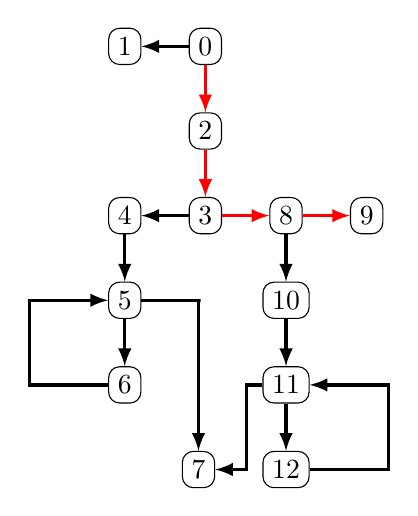
\begin{tikzpicture}[auto,
  start chain = going below,
  node distance = 6 mm,
  %% box/.style = {draw, rounded corners, on chain, align=center},
  %% arr/.style = {very thick, -latex}
]

\node[box] (b0) {0};
\node[box, left=of b0] (b1) {1};
\node[box, below=of b0] (b2) {2};
\node[box, below=of b2] (b3) {3};
\node[box, left=of b3] (b4) {4};
\node[box, below=of b4] (b5) {5};
\node[box, below=of b5] (b6) {6};
% b12 needs to be defined before b7
\node[box, right=of b3] (b8) {8};
\node[box, right=of b8] (b9) {9};
\node[box, below=of b8] (b10) {10};
\node[box, below=of b10] (b11) {11};
\node[box, below=of b11] (b12) {12};
\node[box, left=of b12] (b7) {7};

\draw[arr]  (b0) -- (b1);
\draw[arr, draw=red]  (b0) -- (b2);
\draw[arr, draw=red]  (b2) -- (b3);
\draw[arr]  (b3) -- (b4);
\draw[arr, draw=red]  (b3) -- (b8);
\draw[arr, draw=red]  (b8) -- (b9);
\draw[arr]  (b8) -- (b10);
\draw[arr]  (b10) -- (b11);
\draw[arr]  (b11) -- (b12);
\draw[arr]  (b12.east) -- ++ (1, 0) |- (b11);
\draw[arr]  (b11) -- ++ (-.5, 0) |- (b7.east);
\draw[arr]  (b4) -- (b5);
\draw[arr]  (b5) -- (b6);
\draw[arr]  (b6.west) -- ++ (-1,0) |- (b5);
\draw[arr]  (b5.east) -- ++ (.75, 0) -| (b7.north);


\end{tikzpicture}
  
    }
  \column{.52\linewidth}{
\begin{align*}
  G &= (V, E) \\[10pt]
  V &= \{0, 1, ..., 12\} \\[10pt] 
  E &= \{ (0, 1), (0, 2), (2, 3), (3, 4),\\ 
  & (3, 8), (8, 9), (8, 10), (10, 11),\\
  & (11, 12), (12, 11), (11, 7),\\
  & (4, 5), (5, 6), (6, 5), (6, 7) \}
\end{align*}

Node $9$ is \textbf{\textit{reachable}} from node $0$ by path $((0,2), (2, 3), (3, 8), (8, 9))$.
    }
\end{columns}
  \end{frame}


  \begin{frame}
\frametitle{afl: instrumentation}
Control-flow graph:
\bigskip
\begin{itemize}
  \item{Nodes - \textit{basic blocks} of a program}
    \medskip
  \item{Edges - \textit{control flow} between basic blocks}
      \end{itemize}
  \end{frame}

  
  \begin{frame}[fragile]
    \frametitle{afl: instrumentation}
	  % how we actually build control flow graphs
    \vspace{-.75cm}\lstinputlisting[language={[x64]Assembler}, linerange={6-74}, basicstyle=\tiny\linespread{0.1}, multicols=2]{example.s}
    % highlight that this is asm for foo, compiled for x86_64, in intel syntax, with no optimization
  \end{frame}


  \begin{frame}
    \frametitle{afl: instrumentation}
    \vspace{-.75cm}\centering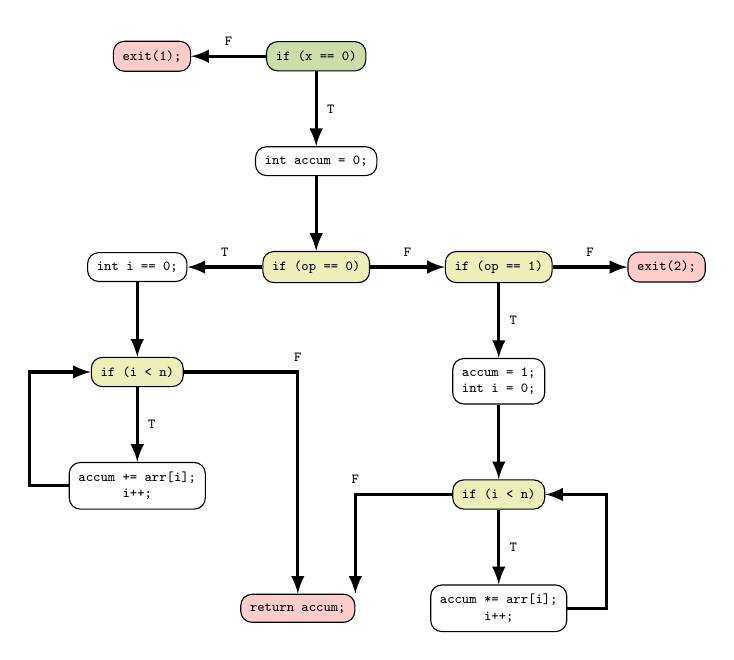
\begin{tikzpicture}[auto,
  start chain = going below,
  node distance = .95 cm,
  font=\tiny\ttfamily
]

\node[decision, fill=pale-green] (b0) {if (x == 0)};
\node[stop, left=of b0] (b1) {exit(1);};
\node[box, below=of b0] (b2) {int accum = 0;};
\node[decision, below=of b2] (b3) {if (op == 0)};
\node[box, left=of b3] (b4) {int i == 0;};
\node[decision, below=of b4] (b5) {if (i < n)};
\node[box, below=of b5] (b6) {
  accum += arr[i]; \\
  i++;
};
% b12 needs to be defined before b7
\node[decision, right=of b3] (b8) {if (op == 1)};
\node[stop, right=of b8] (b9) {exit(2);};
\node[box, below=of b8] (b10) {
  accum = 1; \\
  int i = 0;
};
\node[decision, below=of b10] (b11) {if (i < n)};
\node[box, below=of b11] (b12) {
  accum *= arr[i];\\
  i++;
};
\node[stop, below=of b3, left=of b12] (b7) {return accum;};

\draw[arr]  (b0) -- (b1) node[midway, above]{F};
\draw[arr]  (b0) -- (b2) node[midway, right]{T};
\draw[arr]  (b2) -- (b3);
\draw[arr]  (b3) -- (b4) node[midway, above]{T};
\draw[arr]  (b3) -- (b8) node[midway, above]{F};
\draw[arr]  (b8) -- (b9) node[midway, above]{F};
\draw[arr]  (b8) -- (b10) node[midway, right]{T};
\draw[arr]  (b10) -- (b11);
\draw[arr]  (b11) -- (b12) node[midway, right]{T};
\draw[arr]  (b12.east) -- ++ (.5, 0) |- (b11);
\draw[arr]  (b11) -- ++ (-.75, 0) -| (b7.north east) node[midway, above]{F};
\draw[arr]  (b4) -- (b5);
\draw[arr]  (b5) -- (b6) node[midway, right]{T};
\draw[arr]  (b6.west) -- ++ (-.5,0) |- (b5);
\draw[arr]  (b5.east) -- ++ (.25, 0) -| (b7) node[midway, above]{F};



\end{tikzpicture}

  \end{frame}

\begin{frame}
	\frametitle{afl: instrumentation}
	
	\begin{itemize}
		\item{With source code: drop-in compiler replacement adds some code at each branch point to track edge coverage\footnote{See \url{https://afl-1.readthedocs.io/en/latest/about\_afl.html\#coverage-measurements}}}

		\item{Without source code: on-the-fly instrumentation via binary translator (e.g. QEMU, DynamoRIO, PIN)\footnote{See \url{https://afl-1.readthedocs.io/en/latest/about\_afl.html\#binary-only-instrumentation}}} 
		
		\item{NB: other tools (e.g., \texttt{afl-cov} \cite{aflcov}) necessary for human-interpretable coverage reports from AFL results}
	\end{itemize}
\end{frame}

\begin{frame}
	\frametitle{afl: instrumentation}
	\textbf{Sanitizers} \cite{sanitizers}: compiler passes that insert instrumentation to detect bugs at run-time
	
	\vspace{\baselineskip}
	Examples: \begin{itemize}
		\item{Address sanitizer (ASAN): detects addressability issues, \\e.g., buffer overflows \footnote{See \url{https://github.com/google/sanitizers/wiki/AddressSanitizerAlgorithm}}}
		\item{Memory sanitizer (MSAN): detects use of uninitialized memory}
		\item{Undefined behavior sanitizer (UBSan)}
		% language spec does not define what to do, resulting in variance between compilers and runtimes, e.g. out-of-bounds array access (if bounds can be statically determined)
	\end{itemize}

	\vspace{\baselineskip}
	Sanitizers can be used alone or in combination (see \cite{afl_asannotes}, \cite{githubseclab} for caveats)
\end{frame}


\begin{frame}
	\frametitle{afl: interesting inputs}
	\begin{itemize}
		\item{Input causes a crash}
		\item{Input causes a hang}
		\item{Input causes a new edge to be covered}
	\end{itemize}

\end{frame}

\begin{frame}
	\frametitle{afl: campaign progress}
	\begin{itemize}
		\item{Edge coverage over time}
		\item{Unique crashes / hangs}
	\end{itemize}
\end{frame}

\begin{frame}
	\frametitle{Exercise}
	\begin{enumerate} 
		\item{Run the buffer overflow example.}
		\item{Run the Heartbleed example. Adapted from Michael Macnair's AFL workshop \cite{macnair}.}
	\end{enumerate}
\end{frame}

\section[Research topics]{Research topics in fuzzing \normalsize{(to present)}}
% disclaimer: not exhaustive!

\begin{frame}
	\frametitle{Input generation}
	\textbf{Greybox fuzzing} leverages lightweight instrumentation to prioritize further program exploration. \begin{itemize}
		\item{``Shape aware"}
		\item{Novelty generally based on strategy for selecting next input}
		\item{Examples: AFL (new coverage), AFLFast \cite{aflfast} (unusual path), AFLGo \cite{aflgo} (path close to uncovered basic blocks)}
	\end{itemize}
\end{frame}

\begin{frame}
	\frametitle{Input generation}

	\textbf{Grammar-based fuzzing}: Use specification for input language to produce syntactically valid inputs. Examples: \begin{itemize}
		\item{CSmith \cite{csmith} for compilers}
		\item{Fuzzilli \cite{fuzzilli}, LangFuzz \cite{langfuzz} for JavaScript interpreters}
		\item{H26FORGE \cite{h26forge} for video codecs}
		\item{Grammarinator \cite{grammarinator} for programs with \texttt{antlr}-specified grammars}
	\end{itemize}

\end{frame}

\begin{frame}
	\frametitle{Input generation}
	\textbf{Fuzzing with the help of constraint solvers} 

	\vspace{\baselineskip}
	Concolic fuzzing (``concrete + symbolic")
	\begin{itemize}
		\item{Accumulate constraints on inputs by tracking conditionals during execution}
		\item{Novelty generally based on strategy for appealing to the constraint solver}
		\item{Examples: DART \cite{dart}, SAGE \cite{sage}, CUTE \cite{cute}, EXE \cite{exe}, Driller \cite{driller}, MAYHEM \cite{mayhem}}

	\end{itemize}

	% other techniques do all of their input generation based on information gathered from symbolic execution

\end{frame}

\begin{frame}
	\frametitle{Harnessing}
	\textbf{FUZZ ALL THE THINGS!}

	\begin{itemize}
		\item{Auto-harnessing via program synthesis techniques}
		\item{Handling non-standard inputs (e.g., firmware rehosting)}
	\end{itemize}

\end{frame}

\begin{frame}
	\frametitle{Instrumentation}

	\begin{itemize}
		\item{Source code available: program-specific sanitization}
		\item{Binary only: using dynamic binary instrumentation, binary lifting techniques to support new architectures, add finer-grained instrumentation}
		\item{Improving performance (executions/sec)} % hardware extensions, GPUs
		\item{Running fuzzers at scale (e.g., ClusterFuzz \cite{clusterfuzz})}
		\item{Running fuzzers in ensemble (e.g. EnFuzz \cite{enfuzz}, CollabFuzz \cite{collabfuzz})}
		
	\end{itemize}

\end{frame}

\begin{frame}
	\frametitle{Interesting inputs, campaign progress}

	\textbf{Directed (aka search-based) fuzzing}: measuring novelty and/or progress via alternative metrics to coverage. Examples: \begin{itemize}
		\item{IJON \cite{ijon}}
		\item{FuzzFactory \cite{fuzzfactory}}
		\item{GOLLUM \cite{gollum}}
	\end{itemize}

	\vspace{\baselineskip}
	\centering \includegraphics[scale=.5]{ijon}
\end{frame}

\begin{frame}
	\frametitle{Fuzzer evaluation}
	\textbf{From an art to a science}

	\begin{itemize}
		\item{Reproducibility and statistical significance \cite{klees, seedselection}}
		\item{Comparability: FuzzBench \cite{fuzzbench}}
		\item{Software engineering: libAFL \cite{libafl}}
	\end{itemize}
	
\end{frame}

\begin{frame}
	\frametitle{Conclusion}

	\centering
	\LARGE{What is the ``best" fuzzer?}
	
	\vspace{\baselineskip}
	\pause
	\LARGE{The fuzzer that you've tailored \\to the program under test \\and your analysis objectives!} 
\end{frame}

\appendix
\begin{frame}[allowframebreaks]{References}
	\def\newblock{}
	\bibliographystyle{alpha}
	\bibliography{fuzzing}
\end{frame}

\end{document}
